\chapter{Introduction}
Model-Based Engineering is a recent technology in the domain of electrical and software engineering. In Model-Based Engineering the specification of a system is developed as a model.
%The Unified Modelling Language (UML) offers a large set of Modelling Elements and Diagrams and is also extensible. 
%It can be used to describe almost everything. 
Graphical modelling languages can give a quick and intuitive overview of a system. At the same time one can model very detailed and describe a system bit by bit with formal modelling languages.
Nevertheless in practice creating a model of a system is an effort that needs to pay off in order to be economic.
%modelling is not an end unto itself. 
One way to get a benefit from Model-Based Engineering is to use the design model to automate other tasks in software development. One of those tasks is testing. 
%In Model-Based Testing we try to verify an implementation against its specification that is given as a model. 
In this thesis we will develop an algorithm to automatically generate relevant test cases and even working unit test code from the model. We will focus on UML activity diagrams modelling the control flow and behaviour of a C function in a component based architecture as test model and assume a C function as the implementation to be tested. Since it is not a trivial task to transform a UML activity diagram into C/C++ unit test code we will split the task up into subtasks, specify the interfaces between the different steps, and give algorithms for each step. Due to its generic architecture our algorithm can be adopted for different input models, output languages, coverage criteria, and constraint specification languages by modification of only one or two of the subtasks.
\section{A Real World Problem at Airbus}
\begin{figure}
\label{fig:Act2Code+Tests}
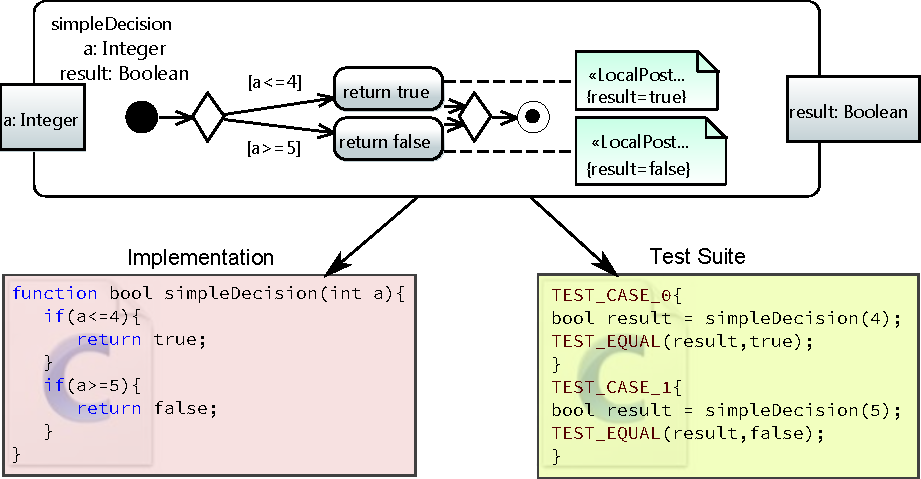
\includegraphics[width=\textwidth]{./pics/Activity2Code+Test2.pdf}
\caption{Example of an activity diagram with a corresponding C implementation and C unit tests}
\end{figure}
At Airbus Buxtehude, Model-Based Engineering shall soon replace the traditional Require-ment--Driven Engineering approach. There are some benefits that we hope to be able to realize with Model-Based Engineering. One benefit is the automatic generation of source code from the design model. Another way to profit from Model-Based Engineering is to use the specification as a test model from which unit test code for the software implementation could be derived. In Figure \ref{fig:Act2Code+Tests} we visualise the idea of using one activity diagram to generate both implementation code and unit test code from it. In the upper part there is a simple activity diagram and below on the left hand side we can see the function implementation that could have been generated from the activity diagram. On the right hand side the generated test suite is shown containing two tests. Each test is testing one control flow path.\\
For modelling behaviour and control flow of C functions UML activity diagrams will be used. The company Atego\textsuperscript{\textregistered} already built a proprietary code generator for Airbus Buxtehude, which generates a folder structure, C source code files, and C header files from a UML model, and fills function bodies with code generated from UML activities. The fact that the code is generated, however, does not make it fault free. We still need to validate the generated code by unit tests. The task in this thesis is to demonstrate how engineers can be supported in building the unit tests for the generated code. We decided to automate the generation of C++ unit tests from UML activity diagrams.\\
%\subsection{Independence of Souce code and Testmodel}
It is common knowledge that one should not generate both the source code and the unit test from the same model. The design model needs to be independent from the test model, otherwise one ends up testing the implementation against itself. That is not meaningful. %We need independence between the implementation and the corresponding unit tests.
%Writing the complete unit test code by hand is cumbersome. 
On the other hand, building a test model to generate unit tests from completely independent from the design model imposes much additional effort. The decision was to share the structure of the activity diagram between code generation and test generation. While the code generation uses procedural C code snippets that are embedded in the model, the test generation only relies on embedded declarative OCL constraints. By using two different programming paradigms as input for code generation and test data generation we assume the generated C implementation to be independent from the generated unit tests.
\section{Outline of this Thesis}
This thesis focuses on generating unit tests from UML activity diagrams with embedded OCL constraints. Our approach is based on graph search algorithms to generate abstract test scenarios. We use symbolic execution and constraint solving to make the test model executable and automatically find useful test data to test the implementation. We put some emphasis on mixed--integer--non--linear arithmetic constraints and will evaluate the limits of state--of--the--art solver implementations.
\subsection{Model Transformations}
We transform a UML activity diagram into a rigorous, executable, mathematical representation. We decided to use multiple subsequent model transformations to carry out this transformation stepwise. In Section \ref{sec:Normalisation} we will specify how the UML and OCL input is transformed to an intermediate representation. During this transformation we can check design rules and ensure properties of the intermediate representation that are necessary in subsequent steps. From this intermediate representation we describe in Section \ref{sec:atcg2Ampl} a model--to--text transformation to \textbf{A} \textbf{M}athematical \textbf{P}rogramming \textbf{L}anguage (AMPL).
\subsection{Symbolic Execution}
In order to make UML activity diagrams executable for test data generation we will transform all relevant constraints embedded in the UML model into AMPL syntax. Executing a certain control flow path in the activity diagram means generating the corresponding mathematical program in AMPL. An AMPL program consists of an AMPL model and AMPL data. One activity diagram will be transformed into one AMPL model and the currently executed control flow path can be specified in the AMPL data.\\
%In order to compute test data for the system under test we will use AMPL (\textbf{A} \textbf{M}athematical \textbf{P}rogramming \textbf{L}anguage). The activity diagram will be represented by arrays of variables and indexed collections of arithmetic constraints. In a data section for the model we can specify which control flow path within the activity diagram we are interested in. From the computed solution to the mathematical program we obtain the test data for the unit tests. 
When building the AMPL model from the activity diagram care needs to be taken that the semantics of the resulting AMPL model corresponds with the semantics the modeller originally had in mind. We support the user by automatically adding constraints that would be cumbersome to make them explicit manually.
\subsection{State--Of--The--Art Constraint Solver Implementations} 
%We generate test data for a control flow path in an activity diagram to be tested by having the corresponding AMPL program solved by a constraint solver. 
A great advantage of a commonly used mathematical programming language is that there are industrial--strength solvers available. By running a state--of--the--art solver the AMPL program corresponding to a possible control flow path in the activity diagram will be solved. From the results of the constraint solver we obtain test data. The generated test data includes possible input arguments for the C function implementing the activity diagram. Also, all expected return values as well as values for class properties before and after the execution of the activity diagram are included.\\
Depending on the problem formulation a suitable solver needs to be selected. Not every solver can solve every AMPL program, and not every AMPL program is an instance of an easy--to--solve problem. An overview of the problems that are considered throughout this thesis can be found in Section \ref{sec:Maths}.
\subsection{Results}
A practical result of this thesis is an Eclipse plug-in automatically generating unit tests from activity diagrams. The plug-in comes with a set of example models. Each example is an instance of a different mathematical problem and thus needs another solver to be solved successfully. Moreover, we performed an industrial case study using a model of the PAX-Call system in Airbus. We added the missing OCL constraints and successfully generated test cases for the largest activity diagram within the model. Finally we experimentally determined the scalability of the implementation.
%To be precice at airbus the decicion was to use UML Activities for modelling behavior and controll flow of C functions for embedded Systems. 
%Basically we want to harvest the benefits from Model Based Engineering by building tool support to generate a test suite for a C function. 
%The generated Test Suite should of course be complete according to some coverage criteria to be selected by the user. 
%And it needs to integrate with the currently used Modelling tools. 
%There is no use in having a Tool working with models when you can not use the models from your standard modelling environment but have to build new models. 

%\subsection{Behavioural Modelling}
%\subsection{Generating Unit Tests from Behavioural Model}
%Explain Model Based engineering at Airbus Buxtehude with Component structure of the software and code generation as well as Test generation from a Model.
%Give the short overview over the complete thesis
\section{Organization}
The rest of this thesis is organized in three chapters. In the chapter \nameref{chap:preliminaries} we will refer to related work (Section \ref{sec:RelatedWork}),%explain the assumed input language (Section \ref{sec:UML}),
give an overview of the theory of mathematical programming and constraint programming (Section \ref{sec:Maths}), and explain the mathematical programming language AMPL.\\
In the chapter \nameref{chap:testgeneration} we first give a short overview of the overall algorithm we are proposing (Section \ref{sec:testgenerationOverview}) and then explain the five subsequent steps of the algorithm (Sections \ref{sec:Normalisation} - \ref{sec:testgenerationUnitTestSynthesis}). Each of them can be viewed as model--to--model, model--to--text, or text--to--model transformation . 
%The last section (Section \ref{sec:testgenerationImplementation}) is about the implementation of the presented algorithm in an Eclipse plug-in.
\\
The chapter \nameref{chap:evaluation} presents the example collection (Section \ref{sec:evaluationAcademicModels}) that has been tested with the implemented Eclipse plug-in and elaborates on the strengths of different solvers. We measured the runtime of our algorithm with different solvers and performed mutation tests with the generated test suits. Also the case study (Section \ref{sec:evaluationCaseStudy}) can be found in this fourth chapter. We experimentally determined the scalability of our implementation within our case study. Finally, we will also sum up a few problems that could not be solved within this thesis (Section \ref{sec:evaluationLimitations}).